\chapter{ТЕОРЕТИЧНИЙ ОГЛЯД ОБРАНИХ ЗАСОБІВ ДОСЛІДЖЕННЯ ТА РОЗРОБКИ }  

\section{BERT}
\subsection{Опис моделі}
BERT - модель, представлена у [3], є однією з найбільш обговорюваних у даний час моделей у сфері обробки природньої мови. Її популярність зумовлена декількома речима. По-перше, модель є надзвичайно універсальною  - вона показує state-of-the-art результати одразу на 11 задачах у сфері обробки природньої мови. По-друге, її легко підтреновувати під конкретну задчу та датасет, що дає можливість використовувати її у різних застосунках. 
\subsection{Як працює модель}
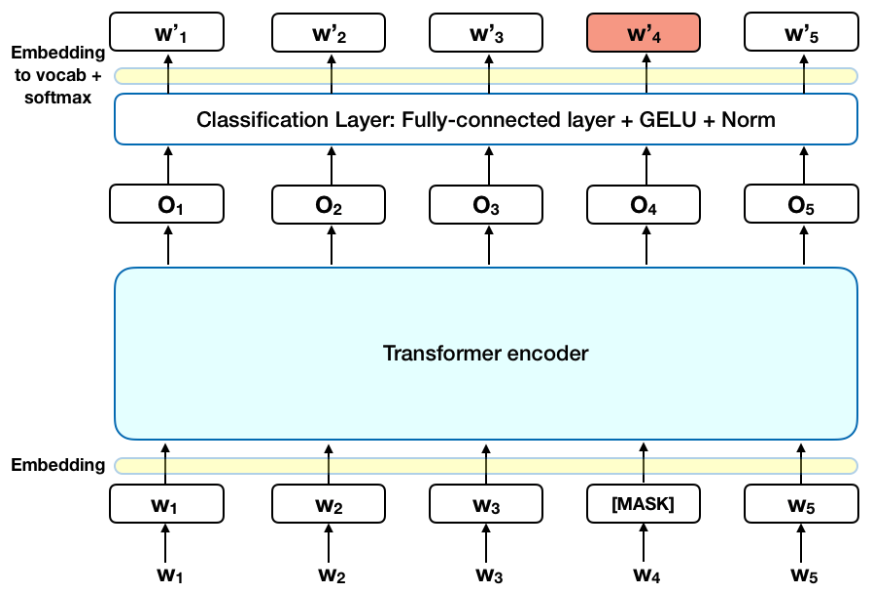
\includegraphics[width=450]{Dissertation/bert_arch.png}\\
\textit{рис. 4. Робота трансформеру.}\\
Основна ідея моделі полягає у тренуванні трансформерів[14] на задачі моделювання мови. Трансформер - це два механізми, один з яких зчитує дані та кодує їх, а інший декодує їх та робить передбачення результату. На відміну від класичних методів роботи з текстами, трансформер не зчитує текст зліва направо, а зчитує все речення разом. Таким чином, ми працюємо з словом та його контекстом, причому контекст слова - це не лише слова перед ним, а й слова після нього. 

Вхідними даними для трансформера є послідовність слів, для яких було пораховано word embeddings[15]. Вихідним значенням є також послідовність векторів, кожний з яких відповідає вхідному слову.

\subsection{Покращення тренування}
Крім трансформерів, BERT також використовує інші підходи для покращення тренування і розуміння контексту слова у реченні. Першим з них є маскування 15\% слів у тренувальних даних. Після трансформації, модель намагається за контекстами сусідніх слів вгадати, яке саме слово було замасковано. 

У тренуванні використовуються пари речень у якості вхідних данних, і модель намагається вгадати друге речення за першим так, ніби це два послідовні речення у одному документі. Під час тренування половина речень є справді послідовними реченнями, а інша половина використовує випадкове речення у якості другого речення.
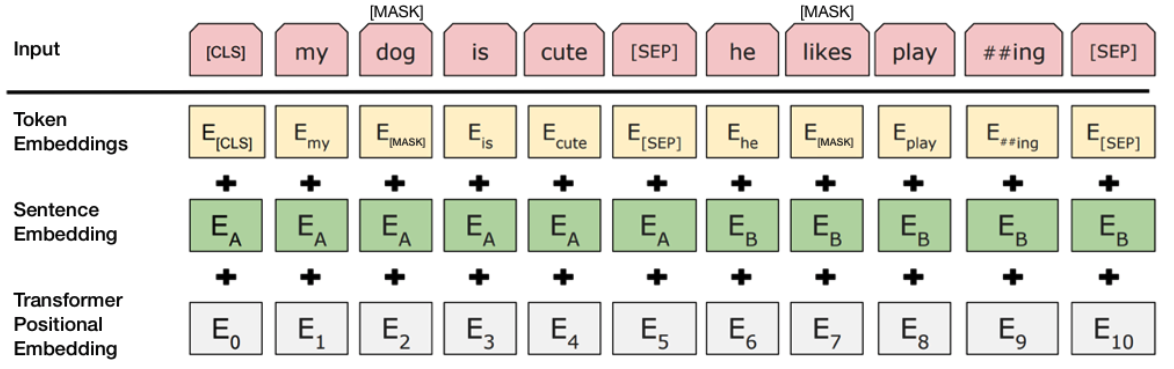
\includegraphics[width = 450]{Dissertation/bert_ex.png}\\
\textit{рис. 5. Як працює тренування на парах речень. }\\
На початок першого речення додається спеціальний токен [CLS], а в кінці кожного речення додаються спеціальні токени [SEP]. Щоб перевірити, чи справді друге речення є пов'язане з першим, ми трансформуємо вхідні данні, та дивимось на значення, що відповідає токену [CLS]. Саме за цим значенням за допомогою функції softmax - це функція $\sigma: \mathbb{R}^{K} \rightarrow \mathbb{R}^{K}$ , що задається формулою
\[
\sigma(\mathbf{z})_{i}=\frac{e^{z_{i}}}{\sum_{j=1}^{K} e^{z_{j}}} \text { for } i=1, \ldots, K \text { and } \mathbf{z}=\left(z_{1}, \ldots, z_{K}\right) \in \mathbb{R}^{K}
\]
 - ми перевіряємо ймовірність того, що ці речення є послідовними.

Ці два підходи поєднується разом під час тренування, з ціллю мінімізувати функцію втрат обох стратегій. Разом, отримуємо модель з понад 375000000 параметрів, що може бути підтренована під різні задачі, пов'язані з природними мовами.
\subsection{Калібрування для інших задач}
 BERT може виконувати багато інших задач у сфері природніх мов [16]. Зазвичай, це досягається додаванням одного додаткового шару у модель. 
 
 Наприклад, задача класифікації текстів вирішується таким саме чином, як і задача розпізнавання наступного речення під час тренування. Додамо спеціальний токен на початку тексту, і за допомогою додаткового шару класифікуємо текст за результатом моделі для цього токену.
 
 Для задачі відповідей на питання, BERT використовує два додаткових вектори, що обозначають початок та кінець відповіді у вихідному тексті.
 
 Для задачі розпізнавання іменованих сутностей, вихідний вектор кожного слова проходить через спеціальний шар-класифікатор. Такий шар класифікує, якому саме типові іменованої сутності  відповідає слово.
 \newpage
\section{Дерево рішень}
\subsection{Опис алгоритму}
Дерево рішень - алгоритм навчання з вчителем, що використовуються у проблемах класифікації. Вперше алгоритм був описаний у [17]. Суть алгоритму полягає у тому, щоб виходячи з тренувальних даних створити бінарне дерево, яке в залежності від деяких параметрів вхідних данних "направляє" їх у ліву чи праву свою гілку. У листках дерева знаходяться відповіді - до якого саме класу належать вхідні дані. \\
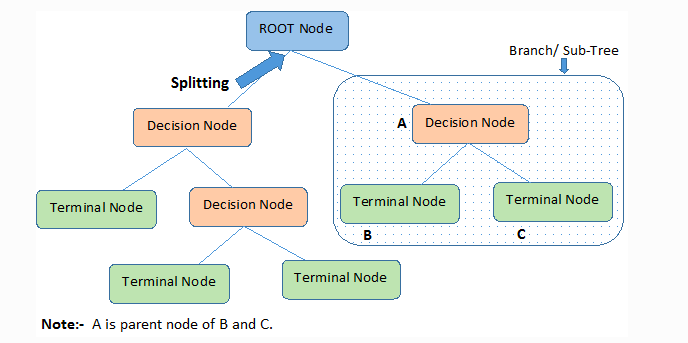
\includegraphics[width = 500]{Dissertation/decision_tree.png} \\
\textit{рис. 6.  Робота дерева рішень}

Перевагою дерева рішень є те, що після тренування, передбачення классу відбувається за час спуску по дереву, тобто 
$\Omega(\log n)$, де n - кількість параметрів моделі. Це дає змогу швидко робити передбачення, використовуючи натреновану модель.
\subsection{Алгоритм побудови}
Дерево рішень будується за наступним алгоритмом[18]. Візьмемо усі тренувальні дані і позначимо їх як кореневу вершину дерева. На кожному кроці роботи алгоритму будемо братий невикористаний параметр з вихідного сету та рахувати його ентропію та додану інформацію. Виберемо параметр, за яким будемо ділити набір даних за допомогою певної метрики. Розділимо набір данних на дві підмножини по цьому параметру та продовжимо рекурсивно роботу алгоритму на цих підмножинах. Будемо продовжувати роботу алгоритму, поки не використаємо усі параметри.

Серед метрик, що використовуються для обрання параметра, за яким будемо ділити, є ентропія, додана інформація, індекс Джині, та додане відношення (описані у [19]).

Ентропія для одного параметру рахується за формулою:
$$
E(S)=\sum_{i=1}^{c}-p_{i} \log _{2} p_{i}
$$, де  S  - поточний стан, a $p_i$ - ймовірність події  i в стані S.
Ентропія для багатьох параметрів рахується за формулою: $$
E(T, X)=\sum_{c \in X} P(c) E(c)
$$, де T - поточний стан, а X- обраний параметр.

Додана інформація - величина, що вказує, наскільки добре даний параметр відділяє дані. 
Вона рахується за наступною формулою: 
$$Information Gain(T,X) = E(T) - E(T, X)$$
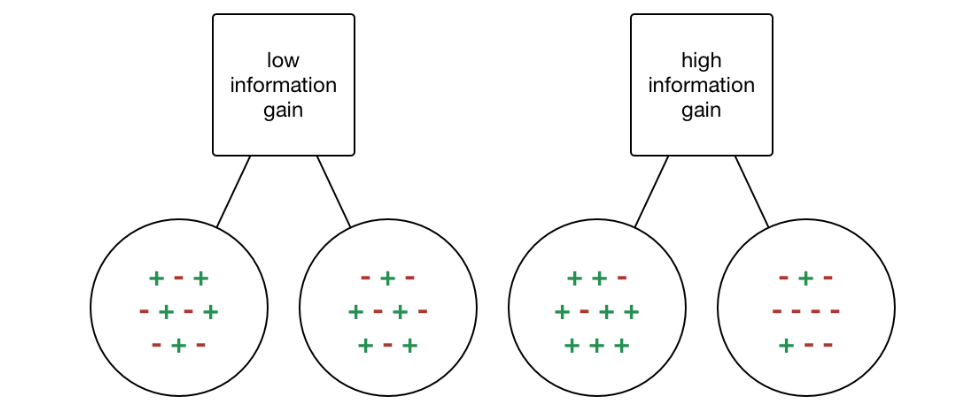
\includegraphics[width=450]{Dissertation/ig.png}\\
\textit{рис 7. Різниця між малою і високою доданою інформацією}

Індекс Джині обчислюється за формулою:
$$
\text {Gini}=1-\sum_{i=1}^{C}\left(p_{i}\right)^{2}
$$
Додане відношення обчислюється за формулою: 
$$
\text {Gain Ratio}=\frac{\text {Information Gain}}{\text {Splittnfo}}=\frac{\text {Entropy}(\text {before})-\sum_{j=1}^{K} \text {Entropy}(j, \text {after})}{\sum_{j=1}^{K} w_{j} \log _{2} w_{j}}
$$



